\documentclass[10pt, a4paper]{report}
\usepackage{amsmath}
\numberwithin{equation}{subsection}
\usepackage{graphicx}
\usepackage{titlesec}
\usepackage{appendix}
\usepackage[french]{babel}
\usepackage{xcolor,graphicx}
\usepackage[top=0.6in,bottom=0.6in,right=1in,left=1in]{geometry}
\usepackage{cite}
\usepackage{tocbibind}
\usepackage{siunitx}
\sisetup{output-exponent-marker=\ensuremath{\mathrm{e}}}
\usepackage{verbatim}
\usepackage{subcaption}
\usepackage{listings}
\begin{comment}
\usepackage{etoolbox}
\makeatletter
\patchcmd{\chapter}{\if@openright\cleardoublepage\else\clearpage\fi}{}{}{}
\makeatother
\end{comment}
%\usepackage[hidelinks]{hyperref}

\begin{comment}
\usepackage{fancyhdr}
\pagestyle{fancy}
\fancyhf{}
\fancyhead[LE,RO]{\thepage}
\fancyhead[LO]{\textit{\nouppercase{\leftmark}}}
\fancyhead[RE]{\textit{\nouppercase{\rightmark}}}
\renewcommand{\chaptermark}[1]{\markboth{#1}{}}
\renewcommand{\sectionmark}[1]{\markright{#1}}
\end{comment}

\usepackage{ifpdf}
\ifpdf
\usepackage[pdftex]{hyperref}
\else
\usepackage{hyperref}
\fi
\renewcommand{\thesection}{\arabic{section}}

%\title{Stage M2 : Calcul du refroidissement du gaz primordial pour la formation des étoiles de population III}
%\author{Miville André}
%\date{Mars 2020}

\begin{document}





\begin{titlepage}
% \pagecolor{blue!10}
\begin{center}
	\begin{minipage}{2.5cm}
	\begin{center}
		
\includegraphics[width=3.0cm,height=1.7cm]{uga.png}
		
	\end{center}
\end{minipage}\hfill
\begin{minipage}{10cm}
	\begin{center}
	\textbf{ Université Grenoble Alpes}\\[0.1cm]
    \textbf{UFR Phitem}\\[0.1cm]
  %  \textbf{-Khouribga-}
% 		\textsc{\uppercase{Université Sultan Moulay Slimane}}
		
% 		\uppercase{éCOLE NATIONALE DES SCIENCES APPLIQUéES KHOURIBGA}
	\end{center}
\end{minipage}\hfill
\begin{minipage}{2.5cm}
	\begin{center}
		
\includegraphics[width=2.3cm,height=2.5cm]{cnrs.png}
	\end{center}

\end{minipage}
%\includegraphics[width=0.6\textwidth]{logo-isae-supaero}\\[1cm]
\textsc{\Large }\\[1.5cm]
{\large \bfseries Rapport de stage de Fin d'\uppercase{é}tudes}\\[0.5cm]
{\large En vue de l'obtention du diplôme}\\[1cm]

{\huge \bfseries \uppercase{Master de physique} \\[0.5cm] }
{\large \bfseries Filière : Astrophysique}
\textsc{\Large }\\[1cm]

% Title
\rule{\linewidth}{0.3mm} \\[0.4cm]
{ \huge \bfseries\color{blue!70!black} Calcul du refroidissement moléculaire du gaz primordial pour la formation des étoiles de population III \\[0.4cm] }
\rule{\linewidth}{0.3mm} \\[1cm]
{\large \bfseries Organisme d'accueil : OSUG IPAG}\\[1cm]
% \includegraphics[width=0.3\textwidth]{logo-isae-supaero}\\[1cm]
% Author and supervisor
\noindent
\begin{minipage}{0.4\textwidth}
  \begin{flushleft} \large
    \emph{\color{orange!80!black}Réalisé par :}\\
    M.~\textsc{Miville} André\\
  \end{flushleft}
\end{minipage}%
\begin{minipage}{0.5\textwidth}
  \begin{flushright} \large
    \emph{\color{orange!80!black}Sous la direction de :} \\
    M.~\textsc{Faure} Alexandre (CNRS)\\
    M.~\textsc{Hily-Blant} Pierre (UGA)\\
  \end{flushright}
\end{minipage}\\[1cm]

\color{blue!80!black}{\large \textit{Soutenu le 15 juin 2020, Devant le jury : }}\\[0.5cm]

\color{black}
\centering
\begin{tabular}{lll}
\large Hervé \textsc{Beust} : & \large UGA IPAG & \large - Président \\[0.1cm]
\large Sébastien  \textsc{Maret} : & \large UGA IPAG & \large - Rapporteur \\[0.1cm]
\large Thierry \textsc{Forveille} : & \large UGA IPAG & \large - Rapporteur
\end{tabular}

\vfill

% Bottom of the page
{\large \color{orange!80!black}{Année universitaire}\\ \color{blue!80!black}2019/2020}

\end{center}
\end{titlepage}





%\maketitle
\renewcommand{\contentsname}{Sommaire}
\renewcommand{\bibname}{Références}



%\addcontentsline{toc}{chapter}{Quelques rappels de Relativité Générale} 
\tableofcontents


\section*{Remerciements}
\addcontentsline{toc}{chapter}{Remerciements} 
Je remercie expréssement mes deux maîtres de stage M. \textsc{Faure} Alexandre et M. \textsc{Hily-Blant} Pierre pour l'encadrement du stage, leurs encouragements, leurs conseils ainsi que leur aide apportée à la réalisation de ce rapport.

Je remercie aussi M. \textsc{Henri} Gilles pour sa disponibilité sans faille à répondre à mes nombreuses interrogations.

Finalement j'exprime ma gratitude envers mes parents qui m'ont légué des valeurs qui se complètent et qui expliquent en outre le succès relatif de mon parcours de vie. À mon oncle Simon qui m'a poussé à faire des études.
 

\section*{Introduction}
\addcontentsline{toc}{chapter}{Introduction} 
\addcontentsline{toc}{section}{Missions effectuées}
\addcontentsline{toc}{section}{Conventions utilisées}
La formation des premières étoiles, dites de population III, a lieu avant l'époque de réionisation, à un décalage vers le rouge cosmologique $\approx$20. Bien que les contraintes observationnelles directes sur la formation de ces premières étoiles soient inexistantes, des contraintes indirectes seront obtenues dans les 10 prochaines années. D'ailleurs, plusieurs interféromètres radio observant la raie de l'hydrogène atomique à 21 cm, décalée vers le rouge, ont d'ores et déjà commencé à accumuler des données, et de futurs instruments tels que SKA, l'E-ELT, ou le JWST, produiront des images du milieu intergalactique neutre et des galaxies à des redshifts $>$10.

Une question fondamentale pour la formation des premières étoiles est celle du refroidissement du gaz baryonique piégé dans les halos de matière noire. De l'efficacité de ce refroidissement dépendra la masse des premières étoiles, et ainsi la rétroaction sur l'évolution de la matière baryonique au cours de la naissance des premières structures. \begin{comment}D'après le modèle $\Lambda $CDM, la nucléosynthèse primordiale crée principalement des atomes d'hydrogène et d'Hélium. Avant les premières étoiles, les molécules régissant le refroidissement moléculaire sont alors simples. Dans mon stage nous nous sommes concentré sur H2. Les détails de la formation de H2, et notamment de ses formes ortho et para, sont donc essentiels.\end{comment}

Il s'agit d'abord de simuler un univers homogène et isotrope en expansion avec un modèle $\Lambda$CDM de la période de recombinaison jusqu'à l'époque de formation des premières étoiles. Ceci nous permet d'avoir des conditions initiales pour le calcul du refroidissement moléculaire où se forment les premières étoiles.

La simulation d'univers homogène et isotrope pour les conditions initiales sur la chimie n'est pas un travail inédit en soi, d'autres chercheurs ont déjà effectué des recherches similaires\textsuperscript{\cite{Coppola} \cite{Flower}}. Mais le rapport de la mission Planck 2018\textsuperscript{\cite{Planck2018}} et de nouvelles données collisionnelles de grande précision offrent l'opportunité d'améliorer et de compléter les résultats existants. 

La problématique de notre sujet demande d'avoir une vue d'ensemble sur différentes spécialités en physique, d'être pluridisciplinaire. La petite équipe n'est pas experte dans tous les domaines. Notamment le modèle $\Lambda CDM$ où il a fallu se mettre à jour. Par conséquent le début du stage a concerné la compréhension dans les grandes lignes de ce modèle, afin de pouvoir l'utiliser en version simplifié et l'appliquer à notre objectif de calcul du refroidissement moléculaire.

Dans ce rapport l'auteur entremêle des généralités -- pour fournir un minimum de contexte --, des justifications théoriques et les résultats préliminaires.
%Par ailleurs l'augmentation continue de la puissance de calcul des processeurs permet l'implémentation de modèles toujours plus évolués.
%Mes maîtres de stage se sont saisi de l'occasion pour se lancer et découvrir cette problématique externe à leur expertise initiale. 


\subsection*{Missions effectuées}

J'ai été amené à revoir les bases de la relativité générale, du transfert de rayonnement, de la mécanique quantique, de la chimie moléculaire, à me documenter sur le modèle $\Lambda$CDM, à redémontrer et fournir les formules utilisées dans les publications de références et de notre modèle, à utiliser le programme RADEX, à programmer en C, Fortran, python, bash, à réaliser un intégrateur Runge Kutta, à interfacer des programmes entre eux, à produire des courbes/graphiques de résultats, à faire des présentations, à écrire un rapport de stage.

%\section*{Quelques rappels de Relativité Générale}


\subsection*{Conventions utilisées}

Dans ce rapport a été utilisé :
\begin{itemize}
	\item[$-$] La convention de signe $(-++)$ en rapport à la classification des signes établi par Misner, Thorne, et Wheeler\textsuperscript{\cite{Signes}}, correspondant respectivement à la définition au signe près du tenseur métrique, du tenseur de courbure et du tenseur d'Einstein. La signature de la métrique utilisée est donc $(+---)$.
	\item[$-$] Les unités SI, pas d'unités naturelles.
	\item[$-$] La définition de la quadrivitesse suivante : $u^\mu = \frac{{\rm d}x^\mu}{{\rm d}\tau}$ avec $\tau$ le temps propre
	\item[$-$] $\rho$ peut être une densité massique ou énergétique (dépend du contexte).
\end{itemize}



\section{Préliminaire : l'Univers en expansion}

\subsection{Le principe cosmologique et la métrique FLRW}
En Relativité Générale, l'équation d'Einstein permet de faire évoluer la forme de l'espace temps -- associé à la métrique et au champ d'accélération gravifique -- en fonction de la distribution d'énergie ou de masse sur cet espace temps. Problème, pour qu'une distribution d'énergie dans l'univers ait un sens, il faut d'abord définir une forme d'univers sur lequel on place les masses. La condition initiale de la forme de l'univers pose alors un certain problème qu'on résoud grâce au principe cosmologique.

En termes simples, le principe cosmologique d'homogénéité et d'isotropie spatiale est l'hypothèse selon laquelle il n'y a pas d'endroit ni de direction privilégiés dans l'espace spatial. On place un observateur cosmique en chacun des points de l'espace spatial 3D et la métrique associée ne dépend pas du point spatial où l'on se situe car ils sont tous équivalents. Points spatiaux car l'univers n'est pas identique à lui même par translation dans le temps. Le temps relié à ces observateurs s'appelle le temps cosmique. Un espace spatial à courbure constante est un espace spatial homogène et isotrope.  La constatation expérimentale de l'expansion de l'univers permet de justifier l'apparition d'un facteur d'échelle dépendant du temps cosmique. La métrique de Friedmann–Lemaître–Robertson–Walker (FLRW) rend compte de ces hypothèses.

En coordonnées généralisées $x= (t,r, \theta, \phi)$ la métrique FLRW avec la signature $(+---)$, se note :

\begin{equation}
\boxed{ c^2 {\rm d}\tau^2 \simeq g_{\mu \nu}dx^{\mu}dx^{\nu} = c^2 {\rm d}t^2 - a(t)^2 \left (\frac{{\rm d}r^2}{1 - k r^2} + r^2 ({\rm d}\theta^2 + \sin^2 \theta \; {\rm d} \phi^2) \right )}
\end{equation}

où $g_{\mu \nu}$ est le tenseur métrique, $t$ est le temps cosmique, $\tau$ le temps propre, $a(t)$ est le facteur d'échelle, $k$ est le facteur de courbure : $k = \{-1,0,1\}$ pour un espace respectivement à courbure ouverte (correspondant à une géométrie hyperbolique), à courbure nulle (correspondant à l'espace euclidien) et à courbure fermée (correspondant à la surface d'une sphère de dimension 4), $t$ est le temps cosmique. Si le facteur de courbure est nul, $\theta$, $\phi$ et $r$ correspondent aux coordonnées sphériques usuelles.

Les observations ne permettent pas encore de se prononcer sur la valeur du facteur de courbure $k$ de l'Univers mais elles suggèrent que la courbure spatiale actuelle de l'espace est plus ou moins nulle $ \kappa \approx 0 \pm [\num{1e-4}]$. $\kappa$ est différent de la courbure scalaire $R$ de l'équation d'Einstein et est relié au facteur de courbure par $\kappa = \frac{k}{a(t)^2}$. Dans ces conditions prendre $k=0$ n'est pas déconseillé\textsuperscript{\cite{Weinberg}} et permet de simplifier les raisonnements et formules. Dans la suite de ce rapport nous nous restreindrons à $k=0$. 
\subsubsection{Distances physiques}
Soient des coordonnées cartésiennes avec un espace plat. Soient deux points au même instant $t_0$ séparés par une distance comobile $\Delta X$. Pour évaluer la distance physique $L$ séparant ces deux points, on peut faire propager un photon les reliant et multiplier le temps de parcours par la vitesse de la lumière pour avoir la-dite distance physique. On a donc un intervalle de genre lumière et on montre sans difficulté que :
\begin{equation}
\boxed{ L=\int\limits_0^{\Delta X} a(t)dx}
\end{equation}
avec \begin{equation}
\boxed{ t=t_0 + \int\limits_0^x a(t')dx'}
\end{equation}
et ainsi de suite pour $t'$.
De sorte qu'au premier ordre il tient que :
\begin{equation} \label{eq:foL}
\boxed{ L \approx a(t_0) \times \Delta X}
\end{equation}
\subsubsection{Décalage vers le rouge cosmologique}
Le décalage vers le rouge $z$ est par définition : 
\begin{equation}
\boxed{1+z = \frac{\lambda_{\mathrm{obs}}}{\lambda_{\mathrm{emit}}}}
\end{equation}

Le décalage vers le rouge cosmologique est le décalage dû à l'expansion de l'univers. En considérant que le nombre de noeuds d'un photon dans une cavité du vide de longeur $L$ à l'instant $t_0$ est conservé au cours du temps, il est montré en utilisant la formule approchée \ref{eq:foL}, l'expression exacte que :
\begin{equation} \label{eq:zC}
\boxed{1+z = \frac{a(t_{pr\acute esent})}{a(t_{\acute emission})}}
\end{equation}

\subsection{\uppercase{é}quation d'Einstein avec la métrique FLRW}
Il est rappelé l'équation d'Einstein :
\begin{equation} \label{eq:EFE}
\boxed{R_{\mu \nu} \ - \ \frac{1}{2} \, g_{\mu \nu} \, R  \  =  \frac{8 \pi G}{c^4} T_{\mu \nu}}
\end{equation}
Où $g_{\mu \nu}$ est le tenseur métrique, $R_{\mu \nu}$ le tenseur de Ricci, $R$ la courbure scalaire de l'espace-temps égale à la contraction du tenseur de Ricci,  $G$ la constante gravitationnelle de Newton, $c$ la célérité de la lumière dans le vide et $T_{\mu \nu}$ le tenseur énergie impulsion.
Que prendre alors pour le tenseur énergie-impulsion ?
\subsubsection{Le fluide parfait}
Les formes d'énergies sont modélisées dans l'univers comme faisant partie d'un fluide parfait exerçant une pression $P$ de densité énergétique $\rho$ au repos par rapport à un observateur cosmique. Son équation qui se déduit de sa formulation en physique classique est : 

\begin{equation} \label{eq:FP}
\boxed{T_{\mu\nu} = (P + \rho) u_\mu u_\nu - P g_{\mu\nu}}
\end{equation}

\subsubsection{Les équations de Friedmann}
En égalisant des deux cotés de l'équation d'Einstein, il se déduit après un long calcul\textsuperscript{\cite{cours_RG1}} les équations de Friedmann :

\begin{equation} \label{eq:F1}
\boxed{H^2 = \frac{8 \pi G}{3}\rho - \frac{kc^2}{a^2}}
\end{equation}
\begin{equation} \label{eq:F2}
\boxed{\dot{H} + H^2 = \frac{\ddot{a}}{a} = - \frac{4\pi G}{3c^2}\left(\rho + 3P\right) }
\end{equation}
Où $H$ est la constante de Hubble dépendante du temps $H=\frac{\dot{a}}{a}$, $\dot{H} = \frac{dH}{dt}$ et $K$
On peut réexprimer la seconde équation grâce à la première en une forme plus pratique qui donne la dérivée de la densité énergétique :
\begin{equation} \label{eq:F3}
\boxed{\frac{{\rm d}\rho}{{\rm d}t} = - 3 H (P + \rho) }
\end{equation}
Si la pression est proportionnelle à la densité : $P= w \rho$ alors \ref{eq:F3} possède une solution analytique :
\begin{equation} \label{eq:F3S}
\boxed{\rho = Cste \times a^{-3(1+w)}}
\end{equation}
Si la densité est composé de deux espèces différentes comme par exemple la densité d'énergie de masse de la matière et celle du champ radiatif alors l'équation \ref{eq:F3} se découple en deux équations indépendantes : Si $\rho = \rho_m + \rho_r$ alors $\frac{{\rm d}\rho_m}{{\rm d}t} = - 3 H (P_m + \rho_m) $ et $\frac{{\rm d}\rho_r}{{\rm d}t} = - 3 H (P_r + \rho_r)$.



\subsubsection{Densité critique}
La densité critique énergétique est la densité telle que l'expansion est nulle pour une courbure nulle ou négligeable. Son expression formelle se comprend de sa définition à partir de l'équation de Friedmann 1 : (voir eq: \ref{eq:F1})

\begin{equation} \label{eq:DEC}
\boxed{\rho_{\rm c}(t) \equiv \frac{3 c^2 H(t)^2 }{8 \pi G} }
\end{equation}

La densité d'énergie d'un certain type est souvent exprimé par son rapport sans dimension avec la densité critique appelé paramètre de densité :

\begin{equation} \label{eq:OD}
\boxed{\Omega(t) \equiv \frac{\rho(t)}{\rho_{\rm c}(t)} }
\end{equation}

\subsubsection{Intégrateur et solutions classiques}
Un intégrateur qui résout l'expansion en fonction du temps a dû être développé.  L'intégrateur est une implémentation de la méthode Runge-Kutta d'ordre 6 en C. Les résultats de notre intégrateur dans des cas d'école simples tels que l'Univers de De Sitter\textsuperscript{\cite{cours_RG1}} et l'Univers d'Einstein-De Sitter\textsuperscript{\cite{cours_RG1}} sont résumés dans la figure ~\ref{fig:UISC}. Ces modèles d'univers sont simples et possèdent une solution analytique. Il s'agit simplement ici de vérifier que l'intégrateur fonctionne. Il n'y a aucun autre intérêt. L'intégrateur reproduit parfaitement les courbes attendues. Le temps cosmique normalisé est le temps sans dimension : $t' = H_0 \times t$. $H_0$ est la constante de hubble actuelle. Pour distinguer les deux courbes, des points discrets ont été tracés au lieu d'une ligne continue.  Le temps nul correspond à actuellement et le facteur d'échelle y est pris à 1($t_0=0, a(t_0)=1$). L'intégrateur remonte dans le temps. On retrouve dans l'univers de poussière d'Einstein-De Sitter que l'univers survit deux tiers du temps de Hubble : $\frac{2}{3H_0}$ 

\begin{figure}[]

\begin{subfigure}{0.5\textwidth}
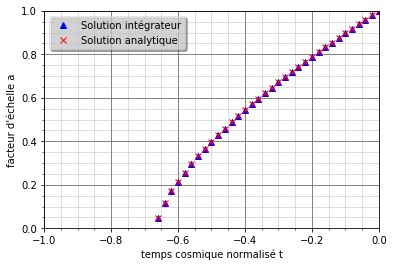
\includegraphics[width=8.0cm,height=6cm]{EDSf.png}
\caption{Univers Einstein-De Sitter}
\label{fig:UEDS}
\end{subfigure}
\begin{subfigure}{0.5\textwidth}
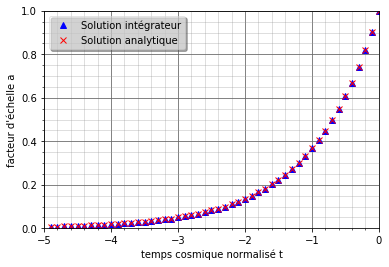
\includegraphics[width=8.0cm,height=6cm]{DSf.png}
\caption{Univers De Sitter}
\label{fig:UDS}
\end{subfigure}

\caption{Comparaison des solutions analytiques et intégrateur}
\label{fig:UISC}
\end{figure}

%\begin{comment}
\makeatletter
\renewcommand\chapter{\thispagestyle{plain}%
\global\@topnum\z@
\@afterindentfalse
\secdef\@chapter\@schapter}
\makeatother 
%\end{comment}

\section{Modèle simplifié inspiré du modèle $\Lambda$CDM}
$\Lambda$ est la constante cosmologique et CDM est l'acronyme de Cold Dark Matter. \begin{comment}C'est une théorie à paramètres. La fameuse matière noire n'est toujours pas identifiée. La valeur de la constante cosmologique est le résultat d'un ajustement. Néanmoins cette théorie permet d'expliquer avec une grande validité diverses constatations astrophysiques. Nous n'avons pas besoin d'en comprendre tous les détails pour poursuivre l'objectif de ce stage.\end{comment}

\subsection{Valeurs des paramètres par la mission Planck 2018}
Le tableau \ref{tab:PI} liste les valeurs utilisées dans notre modèle. Elles sont calculées, fixées ou prises dans le tableau 2 page 15 colonne "TT,TE,EE+lowE+lensing" du papier "Planck 2018 results. VI. Cosmological parameters"\textsuperscript{\cite{Planck2018}}. Les paramètres sont ceux au temps présent actuel $t_0$. 
\begin{table}
\begin{center}
\begin{tabular}{ m{5cm} m{5cm} m{5cm}} 
 \hline
 Description & Paramètre & Valeur numérique\\ 
 \hline
Densité d'énergie noire & $\Omega_\Lambda$ & 6.847e-1±0.0073\\ 
Densité de matière noire et baryonique & $\Omega_m$ & 3.153e-1±0.0073\\ 
Densité de matière noire & $\Omega_{dm}$ & 2.660e-1\\ 
Densité de matière baryonique & $\Omega_b$ & 4.93e-2\\ 
Densité de rayonnement (EM+neutrinos) & $\Omega_r$ & 9.28e-5\\
Densité liée à la courbure spatiale & $\Omega_K$ & 0.000±0.002\\
z équivalent & $z_{eq}$ & 3.402e3±26\\
Température du corps noir & $T_0 [K]$ & 2.7255e0\\ 
Constante de Hubble & $H_0 [km.s^{-1}.Mpc^{-1}]$ & 6.736e1±0.54\\ 
 \hline

\end{tabular}
\end{center}
\caption{Paramètres modèle $\Lambda$CDM simplifié}
\label{tab:PI}
\end{table}

\subsection{La constante cosmologique et l'énergie noire}
L'équation d'Einstein avec constante cosmologique s'écrit:
\begin{equation} \label{eq:EFEL}
\boxed{R_{\mu \nu} \ - \ \frac{1}{2} \, g_{\mu \nu} \, R  \ - \ \Lambda \ g_{\mu \nu} \ =  \frac{8 \pi G}{c^4}  T_{\mu \nu}}
\end{equation}
On peut cependant interpréter la constante cosmologique comme un fluide parfait de densité d'énergie positive constante qu'on appelle énergie noire et de pression négative avec pour équation d'état :
\begin{equation} \label{eq:EEL}
\boxed{P_\Lambda=-1 \times \rho_\Lambda}
\end{equation}
La méthode est de poser un nouveau tenseur énergie-impulsion qui inclut en son sein la constante cosmologique grâce à un changement de variable. On obtient finalement que la densité volumique d'énergie noire vaut :
\begin{equation} \label{eq:DEL}
\boxed{\rho_{\Lambda}  =  \frac{c^4 \Lambda}{8\pi G}}
\end{equation}

\subsection{La matière noire et baryonique froide}
La matière noire est supposée interagir uniquement par gravité. On suppute aussi qu'elle est froide de sorte que seule son énergie de masse compte pour le calcul de la densité d'énergie. 
Dans ce stage, la période d'intérêt fait que la température cinétique de la matière baryonique est constamment inférieure à 10 000K. Cette température est considérée comme froide en comparaison à l'énergie de masse. Pareillement à la température de la matière noire, la température baryonique n'intervient donc pas dans le calcul de la densité d'énergie, seule son énergie de masse compte. Cela revient à considérer que la matière exerce une pression nulle.
En conséquence son équation d'état est :
\begin{equation} \label{eq:EEM}
\boxed{P_m=0 \times \rho_m c^2}
\end{equation}
avec $\rho_m$ la densité de masse de la matière noire et baryonique.
D'après \ref{eq:F3S}, on obtient que :

\begin{equation} \label{eq:DEM}
\boxed{\rho_{\rm m}(t) = \rho_{\rm m}(t_0) \left(\frac{a(t_0)}{a(t)}\right)^3}
\end{equation}

Cette dernière équation peut aussi se retrouver par un raisonnement sur la densité particulaire qui varie comme :
\begin{equation} \label{eq:NP}
\boxed{n(t) = n(t_0) \left(\frac{a(t_0)}{a(t)}\right)^3}
\end{equation}

\subsection{Le champ de rayonnement électromagnétique et les neutrinos}
La découverte du fond diffus cosmologique a eu impact retentissant en cosmologie. Grâce à lui nous pouvons savoir notre vitesse par rapport à ce champ de rayonnement, définissant en quelque sorte un référentiel privilégié, fait rare en relativité générale. Ce "référentiel" n'est autre que celui de l'observateur cosmique ajoutant du crédit au principe cosmologique et à la métrique FLRW. 
\subsubsection{La température de radiation}
Le fond diffus est un rayonnement primordial qui s'est refroidi avec l'expansion et dont la distribution en fréquence se modélise comme un corps noir presque parfait de température T dont la distribution est donnée par la loi de planck. En plaçant des photons dans une cavité du vide de longueur L, on montre fortunément que le refroidissement adiabatique dû à l'expansion d'un corps noir est un corps noir de température amoindrie, de sorte que $T_r$ évolue en $T_{r0} (1+z)$:
\begin{equation} \label{eq:TRRA}
\boxed{T_r(t) = T_r(t_0) \frac{a(t_0)}{a(t)}}
\end{equation}

%\subsubsection{\uppercase{é}quation d'état}
Par le même raisonnement on montre que la densité d'énergie radiative évolue en $\rho_{r0} (1+z)^4$ :
\begin{equation} \label{eq:DER}
\boxed{\rho_r(t) = \rho_r(t_0)  \left({\frac{a(t_0)}{a(t)}}\right)^4}
\end{equation}

Avec la distribution de Planck on trouve le tenseur énergie impulsion du champ radiatif et le résultat bien connnu que la pression radiative vaut le tiers de l'énergie radiative (pour un corps noir) :
\begin{equation} \label{eq:EER}
\boxed{P_r = \frac{1}{3} \times \rho_r}
\end{equation}
Grâce à l'équation d'état on peut utiliser \ref{eq:F3S} pour retrouver \ref{eq:DER} 

\subsubsection{Neutrinos}
Les neutrinos ont des masses nulles ou quasi-nulles et une vitesse égale ou proche de celle de la lumière. Ils peuvent être traités comme des photons, mais l'histoire de l'univers dans sa genèse fait que la densité d'énergie des neutrinos est moindre :

\begin{equation} \label{eq:EDN}
\boxed{\rho_n \approx 0.68 \times \rho_r}
\end{equation}
La prise en compte de la densité énergétique des neutrinos en sus des photons permet de trouver une bonne estimation de $\Omega_{ro}$.
\subsection{Intégrateur et solution de l'expansion}
Au vu de ce qui a été dit depuis le début, l'équation de Friedmann 1 (\ref{eq:F1}) s'écrit pour nos conditions :

\begin{equation} \label{eq:ELCDM}
\boxed{a' = \sqrt{\Omega_{\Lambda}*a^2+\Omega_{m0}/a+\Omega_{ro}/a^2}}
\end{equation}
avec $a'$ la dérivée par rapport au temps cosmique normalisé. Le temps cosmique normalisé est le temps sans dimension : $t' = H_0 \times t$.  Le temps nul correspond à actuellement et le facteur d'échelle y est pris à 1 ($t_0=0, a(t_0)=1$).  On obtient la figure \ref{fig:ULCDM} après avoir intégré \ref{eq:ELCDM}. L'intégrateur remonte dans le temps. L'Univers survit une portion d'environ 0.95 du temps de Hubble.

\begin{figure}[]
\centering
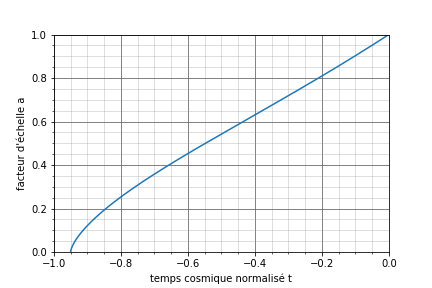
\includegraphics[width=12.0cm,height=9cm]{LCDMf.png}
\caption{Univers $\Lambda$CDM simplifié}
\label{fig:ULCDM}
\end{figure}
 

%\section{L'époque de recombinaison}
\section{\uppercase{é}changes d'énergie entre photons et électrons}
\subsection{La température baryonique}
On suppose que la matière interagit suffisament par collision pour justifier une hypothèse simplificatrice, celle d'une température baryonique $T_b$. Pleinement justifiée aux grands $z$, cette hypothèse est discutable aux petits $z$ où la densité devient faible.
\subsubsection{Refroidissement adiabatique dû à l'expansion}
L'hypothèse de De Broglie est employée afin d'appliquer le même raisonnement que celui de la conservation des noeuds d'une longeur d'onde dans une cavité. Il vient que $T_b$ évolue en $T_{b0} (1+z)^2$:

\begin{equation} \label{eq:RTB}
\boxed{T_b(t) = T_b(t_0) \left(\frac{a(t_0)}{a(t)}\right)^2}
\end{equation}

\subsection{Processus Compton}
C'est le processus de diffusion d'un photon sur un électron libre, il a une importance capitale en cosmologie à cause de sa grande section efficace. Cette dernière est inversement proportionnelle au carré de la masse, la diffusion d'un photon avec un proton peut donc être négligée. On rappelle les résultats principaux. Dans le référentiel de l'électron au repos, le photon de longeur d'onde $\lambda$ arrivant sur l'électron définit une direction privilégiée. Dans cette configuration, l'électron ne peut que gagner de l'énergie. On note $\theta$ l'angle de déviation du photon par rapport à sa propre direction.
La variation de longeur d'onde vaut :
\begin{equation} \label{eq:VLO}
\boxed{\Delta\lambda=\frac{h}{m_e c}(1 - \cos \theta)}
\end{equation}

 Le premier ordre non trivial de l'électrodynamique quantique nous dit que la section efficace différentielle non polarisée vaut (formule de Klein-Nishina) :
\begin{equation} \label{eq:QED}
\boxed{\frac{d\sigma}{d\Omega} = \frac{1}{2} r_e^2 \left(\frac{\lambda}{\lambda'}\right)^{2} \left[\frac{\lambda}{\lambda'} + \frac{\lambda'}{\lambda} - \sin^2(\theta)\right]}
\end{equation}


Si l'électron n'est pas au repos, on peut toujours faire un changement de référentiel pour avoir l'électron au repos et appliquer la théorie du processus Compton, puis faire un changement de référentiel inverse pour revenir au référentiel initial où l'électron se meut. L'électron ou le photon peut alors avoir gagné ou perdu de l'énergie. On désigne par Processus Compton Inverse le cas où l'électron transfert de son énergie aux photons.

La diffusion Thompson est la limite basse énergie de la diffusion Compton. Dans cette approximation, le photon accélère une particule chargée qui rayonne. Ce rayonnement est alors interprété comme étant la diffusion du photon sur la particule chargée. 
 
\subsection{Fraction d'ionisation $x_e$}
Par définition :
\begin{equation} \label{eq:XE}
\boxed{x_e= \frac{n_e}{n_p+n_H}}
\end{equation}
On peut utiliser dans un premier temps la loi de Saha-Langmuir valable pour une ionisation faible :
\begin{equation} \label{eq:XESL}
\boxed{\frac{n_{i+1} n_e }{n_i} = \frac{2 Z_{i+1}}{Z_i} \left( \frac{2\pi m_ek_bT}{h^2}\right)^{\frac{3}{2}} \exp(\frac{-\chi_i}{k_bT})}
\end{equation}
Son utilisation ici est abusive car la fraction d'ionisation est proche de l'unité à 10000K pour l'hydrogène. Pour les résultats préliminaires il a été choisi de prendre une fraction d'ionisation constante égale à 4e-4\textsuperscript{\cite{Flower}}.

Où $\chi_i$ est le potentiel d'ionisation pour ioniser de nouveau un atome déjà ionisé $i$ fois, $Z_i$ est sa fonction de partition. Cette loi permet d'obtenir la fraction d'ionisation d'un gaz d'hydrogène à la température $T$ avec $\chi_H=13.6 eV$ :
\begin{equation} \label{eq:XE}
\boxed{\frac{x_e^2}{1-x_e} = \frac{1}{n_p+n_H} \left( \frac{2\pi m_ek_bT}{h^2}\right)^{\frac{3}{2}} \exp(\frac{-\chi_H}{k_bT})}
\end{equation}

\subsection{Chauffage des électrons par les photons}

Pour calculer les échanges d'énergies entre les températures baryoniques et de rayonnement on montre que \textsuperscript{\cite{PEEBLESBOOK}} : 
\begin{equation} \label{eq:ITBTR}
\boxed{\frac{dT_b}{dt} = \frac{8\sigma_Ta_rT_r^4(T_r-T_m)}{3m_ec}\frac{x_e}{1+x_e}}
\end{equation}

 où $\sigma_T = \frac{8\pi} 3 \left(\frac{q^2}{4\pi\varepsilon_0mc^2}\right)^2$ est la section efficace de Thompson = 6.652...e-29 $[m^2]$ pour l'électron, $m_e$ la masse de l'électron, $a_r = \frac{8 \pi^5 k^4}{15 h^3 c^3}$ = 7.565...e-16 $[J.m^{-3}.K^{-4}]$ la constante de rayonnement qui relie la densité d'énergie radiative d'un corps noir à sa température radiative et $x_e$ la fraction d'ionisation.

Du fait de cette interaction, la distribution en fréquence des photons n'est plus exactement celle d'un corps noir.   

\subsection{Paramètre $z_{eq}$}
Par définition, il correspond au décalage vers le rouge cosmologique où la densité énergétique de rayonnement est égale à celle de la matière. Par conséquent, on obtient une autre estimation du paramètre $\Omega_{ro} = \frac{\Omega_{m}}{1+z_{eq}}$. $z_{eq} = 3402$ voir tableau \ref{tab:PI}. La température baryonique est environ égale à la température de rayonnement car le terme compensateur Compton est très important : $T_b \approx T_r$ de sorte que l'on utilise cette condition intiale dans notre programme.

\subsection{Intégrateur et évolution des températures}\label{IEEDT}
On néglige pour l'instant l'interaction des photons avec les molécules et atomes. Au vu de ce qui a été dit, la température baryonique évolue comme (à partir de \ref{eq:RTB} et \ref{eq:ITBTR}):

\begin{equation} \label{eq:EERT}
\boxed{\frac{dT_b}{dt} = -2H(t)T_b+\frac{8\sigma_Ta_rT_r^4(T_r-T_m)}{3m_ec}\frac{x_e}{1+x_e}}
\end{equation}

et la température radiative comme (à partir de \ref{eq:TRRA}) :

\begin{equation} \label{eq:EERR}
\boxed{\frac{dT_r}{dt} = -H(t)T_r}
\end{equation}

Après avoir intégré \ref{eq:EERT} et \ref{eq:EERR}, on obtient la figure \ref{fig:T}. Elle résume les résultats de notre intégrateur pour différentes fractions d’ionisation supposées constantes en fonction de z.

\begin{figure}[]
\centering
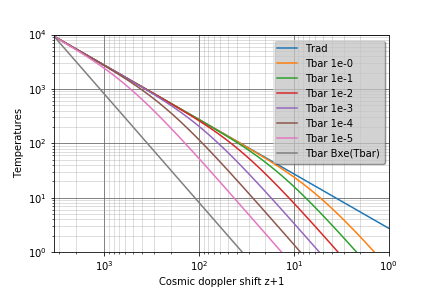
\includegraphics[width=12.0cm,height=9cm]{Temperatures.png}
\caption{\uppercase{é}volution des températures baryonique et de radiation pour différentes fractions d'ionisation}
\label{fig:T}
\end{figure}

\section{Réseau $\&$ molécule H2}
\subsection{Population $\&$ réseau}
Les atomes et molécules considérés pour un modèle possèdent des états d'énergie interne outre leur énergie cinétique qui sont décrits par un certain jeu de nombres quantiques. Le but est de trouver la densité particulaire de chaque espèce dans chaque configuration quantique donnée. Cette dernière densité est aussi égale à la densité totale de l'espèce, fois sa proportion ou population dans l'état quantique. Les densités sont décrites par des équations différentielles qui forment un réseau.\bigskip
\large

Listons les termes sources et puits susceptibles de faire varier les densités particulaires de la molécule/atome dans l'état quantique décrit par le jeu de nombres $i$, $\frac{dn_i}{dt}$ en $[s^{-1}.cm^{-3}]$ :\\

\begin{enumerate}
	\item Les désexcitations radiatives spontanées : $\sum\limits_{j>i} n_jA_{ji}-n_i\sum\limits_{j<i} A_{ij}$
	\item Les absorptions et les émissions stimulées : $\sum\limits_{j<i} n_jB_{ji}J_{ij}+\sum\limits_{j>i} n_jB_{ji}J_{ji}-n_i\sum\limits_{j<i}B_{ij}J_{ij}$
	\item Les excitations et désexcitations collisionnelles avec chaque collisionneur p : \\ $\sum\limits_p\left(n_p\sum\limits_{j<i} n_j C_{ji}-n_pn_i\sum\limits_j C_{ij}+n_p\sum\limits_{j>i}n_j C_{ji}\right)$
	\item Une dilution due à l'expansion du volume : $-3Hn_i$\\
	\item Les termes de réactions chimiques formant ou détruisant l'espèce dans un état quantique donné.
\end{enumerate}
\medskip
\normalsize
La température radiative intervient dans l'expression des moyennes de l'intensité $J_{ij}$, tandis que la température baryonique intervient implicitement dans les taux de collisions $C_{ij}$. 

\subsubsection{\uppercase{é}quilibre statistique, état stationnaire et ETL}
Si l'on fixe une température radiative et cinétique et qu'on laisse le système évoluer de lui-même, les conditions initiales des populations disparaitront et le système se stabilisera vers les densités de l'équilibre statistique et n'évoluera plus. Par conséquent l'équilibre statistique est aussi un état stationnaire. À l'équilibre thermodynamique local (ETL), la température radiative est égale à la température baryonique.

\subsection{Relation entre coefficients collisionnels}
Lorsque les rapports de population sont dominés par les collisions, on doit retrouver des rapports donnés par la loi de Boltzmann. Comme les coefficients décrivent des propriétés intrinsèques à un couple de collisionneurs, les relations suivantes sont invariablement vraies, $w_u$ désignant la dégénérescence de l'état:
\begin{equation} \label{eq:DB}
 \boxed{C_{lu} = C_{ul}\frac{w_u}{w_l}\exp{\frac{-E_{ul}}{k_b T_{kin}}}}
\end{equation}


%\subsection{\uppercase{é}léments de transfert de rayonnement}



\subsection{Le programme RADEX}
RADEX\textsuperscript{\cite{RADEX}} est un programme livré avec le code source qui résout l'équilibre statistique du réseau (les points 1-3 des termes impactant les populations du tableau précédent), i.e. avec les dérivées temporelles des densités particulaires nulles. Il modélise la partie transfert de rayonnement avec une probabilité d'échappement du photon. Le logiciel est capable de fonctionner sans équilibre thermodynamique local et peut prendre ainsi en compte une température radiative différente de la température baryonique. C'est un code très utilisé dans la communauté astrophysique et est utilisé dans ce stage. La capacité de RADEX à modéliser une probabilité d'échappement du photon n'est pas utilisé. Premièrement parce que nous n'avons pas affaire à un nuage mais à du gaz en expansion qui occupe tout l'univers. Deuxièmement la problématique n'est pas la même. Le logiciel est utilisé pour calculer l'intensité des raies issues d'un nuage éventuellement optiquement épais. Dans notre cas, nous nous intéressons uniquement aux populations que retourne RADEX dans un petit volume local d'épaisseur optique infinitésimale. On morcèle un nuage aux petits volumes locaux par exemple. Comme le gaz est en expansion dans un univers homogène et isotrope, la question du lieu de ce petit volume ne se pose pas.     
\subsection{La molécule $H_2$}
La molécule est modélisée en première approximation comme un rotateur rigide -- deux protons fixés par une tige rigide -- et comme un oscillateur harmonique -- la tige est le ressort. Deux nombres quantiques (j et v) décrivent les états rovibrationnels du système.  
\subsubsection{Forme ortho et para}
La molécule de dihydrogène possède deux isomères de spin nucléaire. Une configuration où les moments cinétiques intrinsèques des protons sont parallèles, la forme ortho, et une autre où ils sont anti-parralèlles, la forme para. En réalité cette description est trop simpliste, il faut avoir une approche de mécanique quantique avec le spin nucléaire total. Il y a deux cas possibles : le spin nucléaire total I vaut 1 dégénéré 3 fois avec une projection de la base de spins dans une direction quelquonque valant {-1,0,1} -- la forme ortho -- ou le spin nucléaire total I est nul et dégénéré une seule fois -- la forme para. Les transitions radiatives spontanées entre les deux formes sont fortement interdites -- les temps caractéristiques des ces transitions sont plus élevés que l'âge de l'univers. En revanche les dés/excitations collisionnelles réactives permettent de passer entre les deux formes (par exemple la collision de H2 avec H). 
\subsubsection{Rapport ortho para}
Il est possible de calculer le rapport théorique ortho para pour du dihydrogène à l'équilibre thermodynamique à la température $T$ grâce à la loi de Boltzmann :
\begin{equation} \label{eq:EROP}
\boxed{r(o/p) = \frac{Z_o}{Z_p}}
\end{equation}
avec $Z$ la fonction de partition définie par :
\begin{equation} \label{eq:EZ}
 \boxed{Z = \sum\limits_i g(E_i) \ \exp\left(\frac{-E_i}{k_bT}\right)}
\end{equation}
 
$Z_o$ désignant alors la fonction de partition avec seulement les états d'énergie dans la forme ortho et $Z_p$ défini similairement avec la forme para. $g(E_i)$ est la dégénérescence du niveau d'énergie $E_i$.


\subsection{Intégrateur et rapport ortho para}

La figure \ref{fig:ROP} montre le rapport ortho-para calculé à différents $z$ par l'intégrateur et au programme RADEX. RADEX prend en arguments d'entrée les températures calculées par l'intégrateur ainsi que les densités de collisionneurs. Il s'agit ici des protons et des atomes d'hydrogène. RADEX a aussi besoin d'un fichier d'information sur la molécule $H_2$ et pour ses multiples collisionneurs lui indiquant les niveaux d'énergie et les taux de collisions calculés sur une plage de températures. La densité des atomes d'hydrogène a été prise en considérant que l'ensemble de la matière baryonique est sous forme d'atomes d'hydrogène, ainsi :
\begin{equation} \label{eq:NHT0}
 \boxed{n_H(t_0) = \frac{\Omega_{b} \rho_c}{m_H c^2}= \frac{\Omega_{b}}{m_H c^2}\frac{3 c^2 H_0^2 }{8 \pi G} }  
\end{equation}
et
\begin{equation} \label{eq:NH}
\boxed{n_H(t) = n_H(t_0) \left(\frac{a(t_0)}{a(t)}\right)^3 = n_H(t_0) (1+z)^3} 
\end{equation}

 Dans ce stage nous nous sommes placés à l'équilibre statistique car nous utilisons RADEX pour calculer les populations. Cette approche est justifié lorsque le temps dynamique $\frac{1}{H(t)}$ est supérieur au temps pour atteindre l'équilibre statistique. 

\begin{figure}[]
\centering
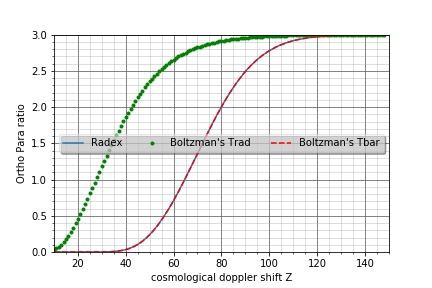
\includegraphics[width=14.0cm,height=9cm]{rop.png}
\caption{Rapport ortho para}
\label{fig:ROP}
\end{figure}

La série de points verts Boltzmann $T_r$ correspond au rapport théorique qu'on obtiendrait avec Boltzmann en prenant la température radiative $T=T_r(z)$.
La série de tirets oranges Boltzmann $T_b$ correspond au rapport théorique qu'on obtiendrait avec Boltzmann en prenant la température baryonique $T=T_b(z)$.
Enfin les points rouges correspondent à la courbe obtenue par Flower et Pineau des Forêts (2000) dans leur modèle. 
Leur rapport ne descend pas vers zéro. Cela vient du fait qu’ils ne résolvent pas les équations de l’équilibre statistique. Aux faibles $z$, quand la densité et la température baryonique deviennent faibles, le temps de désexcitation devient plus grand que le temps dynamique. Ainsi les populations de l'équilibre statistique que l'on calcule avec RADEX n'ont jamais le temps de s'établir, c'est pourquoi le rappport ortho para semble geler vers une valeur non nulle (de l’ordre de 0.3) avec leur modèle. Les différences aux $z \approx 50 - 100$ sont par contre la conséquence d'un modèle physique différent : pas de $\Lambda CDM$, paramètres non égaux, etc...

\section{Refroidissement/réchauffement moléculaire}
\subsection{\uppercase{é}volution de l'énergie cinétique et température baryonique}
Nous ne pouvons définir une température thermodynamique de notre système global prenant en compte l'Hamiltonien total, comme l'énergie potentielle des états internes et gravitationnels, l'énergie cinétique et l'énergie radiative. Par contre nous pouvons définir une température cinétique locale, celle de la distribution des vitesses de Maxwell relié à l'énergie cinétique volumique locale. On suppose que toutes les espèces possèdent la même température cinétique, l'hypothèse se justifie à l'aide de l'argument de la thermalisation de la matière, induite par collisions avec les électrons. 
\bigskip
\large

Listons les termes sources et dissipatifs susceptibles de faire varier l'énergie cinétique volumique locale à l’état stationnaire $\frac{dE_{CV} }{dt}$ en $[J.s^{-1}.cm^{-3}]$ :\\

\begin{enumerate}
	\item La diffusion Compton, de manière générale, la diffusion des photons avec la matière baryonique (voir sections précédentes).
	\item Réchauffement par désexcitations collisionnelles avec chaque collisionneur p\textsuperscript{\cite{RADEX} \cite{KWO}} :\\ $\sum\limits_p\sum\limits_{j>i}\sum\limits_i n_p n_j C_{ji}E_{ji}$
	\item Refroidissement par excitations collisionnelles avec chaque collisionneur p\textsuperscript{\cite{RADEX} \cite{KWO}} :\\ $-\sum\limits_p\sum\limits_{j>i}\sum\limits_i n_p n_j C_{ij}E_{ij}$
	\item Perte d'énergie cinétique due à l'expansion de la longueur d'onde (hypothèse de De Broglie): $-2H E_{CV}$
	\item Pertes volumiques dues à l'expansion du volume : $-3H E_{CV}$
	\item Les termes de réactions chimiques exo/endothermique provenant des créations/destructions de molécules.
\end{enumerate}
\medskip
\normalsize
Les désexcitations radiatives interviennent indirectement en modifiant les populations et l'intensité radiative.

Un calcul classique de théorie cinétique des gaz permet de relier l'énergie cinétique volumique $E_{CV}$ à la température cinétique $T_C$ et les densités particulaires des m espèces (par exemple nH et nH2) :
\begin{equation} \label{eq:ECTC}
 \boxed{E_{CV} = \sum\limits_m  \frac{3 n_m k_b T_C}{2}}
\end{equation}
Ainsi, grâce aux termes des listes précédentes, le nécessaire est là pour calculer la variation de la température cinétique des $m$ atomes/molécules :
\begin{equation} \label{eq:VTC}
 \boxed{\frac{dT_C }{dt} = \frac{d}{dt}\left(\frac{E_{CV}}{\sum\limits_m  \frac{3 n_i k_b}{2}}\right)}
\end{equation}

Les formules 2 et 3 avec les $C_{ij}$ de la liste précédente ne font pas apparaître explicitement les coefficients d'Einstein. Elles s'interprètent comme suit. Une excitation collisionnelle pompe de l'énergie cinétique et la transforme en énergie liée aux états quantiques. Par conséquent il s'agit d'un refroidissement. À l'inverse, une désexcitation collisionnelle transfert de l'énergie liée aux états quantiques en énergie cinétique, constituant ainsi un chauffage. En fesant le bilan de ces deux termes, on obtient le refroidissement/réchauffement net. Cette formule désigne un refroidissement local qui peut se convertir directement en un accroissement ou une diminution de la température cinétique.

\begin{comment}
 Dans le cadre du refroidissement d'un nuage, l'exercice est différent, on cherche l'énergie qui sort du nuage. L'énergie sortante est sous forme radiative et provient de désexcitations spontanées ou induites des états quantiques. Cette énergie n'est pas convertissable directement en accroissement ou diminution de la température cinétique locale, car l'énergie sortante ne provient pas du réservoir d'énergie cinétique mais du réservoir d'énergie liée aux états quantiques. Intuitivement, à l'équilibre statistique, lorsque l'on a laissé les populations se stabiliser au temps$ t=\infinity$ formant un état stationnaire (les populations sont alors indépendantes de la population au temps $t=0$), nous avons une dépendance mathématique entre les populations et les températures radiatives et baryonique, de sorte qu'il y a un lien entre le réservoir d'énergie liée aux états quantiques et le réservoir d'énergie cinétique. 
\end{comment}

\subsection{Pouvoir de réchauffement/refroidissement}
Si l'on divise le refroidissement net par la densité de collisionneur et par la densité du collisionné, on obtient une quantité s'assimilant au pouvoir de refroidissement en [$erg.s^{-1}.cm^{3}$]. La figure \ref{fig:CPfinal} montre le refroidissement que l'on calcule grâce à RADEX pour un gaz à la température cinétique T et à température du champ radiatif externe nul. Les résultats obtenus ont été comparés à la figure 1 du papier de Glover et Abel \textsuperscript{\cite{Glover}}. Le graphe labellisé H est obtenu avec un fichier de collision de H2 avec H (Lique et al. (2015))\textsuperscript{\cite{Lique}} contenant les 54 états rovibrationnels (v=0-3, j=0-17) de la molécule H2. Le graphe labellisé H+ est le refroidissement de H2 avec H+ mais obtenu avec un fichier de collisions de H2 avec H et H+ (Gerllich 1990)\textsuperscript{\cite{Gerlich}} contenant les 9 états rotationnels (j=0-8) de la molécule H2. La densité de H+ a été prise à 1e-4 fois la densité H. Les rapports de densités sont importants pour établir les populations même si ultimement on divise par les densités.\\
On ne remarque pas de différences entre les courbes calculant le refroidissement de H2 avec H+. C'est parce que les deux équipes ont utilisé le même fichier de collision (Gerllich 1990). Nous devions avoir de nouvelles données pour cette collision (Tomas Gonzales-Lezana et al. en préparation) mais malheureusement elles sont toujours en cours de calcul.
Concernant les courbes calculant le refroidissement de H2 avec H, on remarque que notre courbe avec les nouvelles données de collisions (Lique et al. (2015)) montre un refroidissement de 10\% à 40\% supérieur par rapport à la courbe GAHWF07 de Glover \& Abel qui utilise des données de Wrathmall \& Flower (2007). Ceci est dû au fait que les nouvelles données de collisions (Lique et al. (2015)) incluent les conversions ortho/para qui étaient interdites dans les anciens calculs.

\begin{figure}[]
\centering
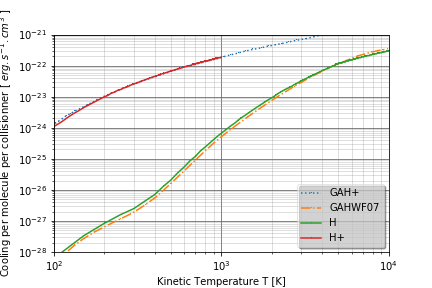
\includegraphics[width=14.0cm,height=9cm]{CPfinal.png}
\caption{Pouvoir de refroidissement de H2 en fonction des différents collisionneurs}
\label{fig:CPfinal}
\end{figure}

\subsection{Réchauffement du gaz en expansion par H2}
Les figures \ref{fig:ZCOOL1} et  \ref{fig:dTCOOL1} montrent le réchauffement collisionnel du gaz par H2 avec H et H+ et son impact sur la température calculé à différents $z$ grâce aux données déduites du modèle par l'intégrateur et au programme RADEX. La densité de H2 a été prise à un rapport constant pour simplifier de 6.3e-7 fois la densité de H\textsuperscript{\cite{Galli} \cite{Flower}}.   
\begin{figure}[]
\centering
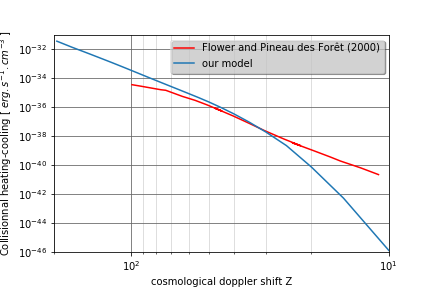
\includegraphics[width=14.0cm,height=9cm]{Zcoolfinal.png}
\caption{Réchauffement net par collision de H2 avec H et H+}
\label{fig:ZCOOL1}
\end{figure}

\begin{figure}[]
\centering
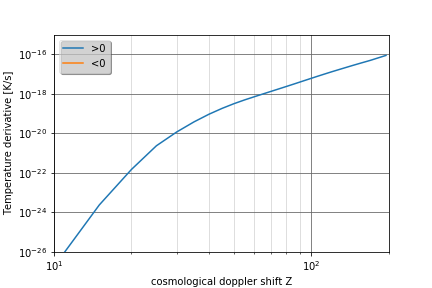
\includegraphics[width=14.0cm,height=9cm]{dTcoolfinal.png}
\caption{Impact du réchauffement sur la température}
\label{fig:dTCOOL1}
\end{figure}
Le temps de Hubble est d'environ 4e17 secondes. Lorsqu'on intègre entre $z=200$ et $z=10$ le réchauffement induit une augmentation d'environ 0.01 K. C'est pourquoi il est tout à fait justifié de négliger la contribution du réchauffement moléculaire dans la partie \ref{IEEDT}


%\subsection{Réchauffement du gaz par HD}
%La figure \ref{fig:ZCOOL} montre le réchauffement collisionnel du gaz par H2 avec H et H+ calculé à différents $z$ grâce aux données déduites du modèle par l'intégrateur et au programme RADEX. La densité de H2 a été prise à un rapport constant pour simplifier de 6.3e-7 fois la densité de H\textsuperscript{\cite{Galli} \cite{Flower}} .  







\begin{comment}
\subsection{Réchauffement/Refroidissement}
Dérivons le refroidissement et le réchauffement pour une seule molécule en présence de p collisionneurs dans le cas stationnaire, pour un champ de rayonnement isotrope en négligeant les termes 4 et 5 de la  section 0.4.1.

On a que : $0=\sum\limits_{j>i} n_jA_{ji}-n_i\sum\limits_{j<i} A_{ij}+\sum\limits_{j<i} n_jB_{ji}J_{ij}+\sum\limits_{j>i} n_jB_{ji}J_{ji}-n_i\sum\limits_{j<i}B_{ij}J_{ij}+\\
\sum\limits_p\left(\sum\limits_{j<i}n_p n_j C_{ji}-n_pn_i\sum\limits_j C_{ij}+n_p\sum\limits_{j>i}n_j C_{ji}\right)$

Les populations ne changent pas, cela permet de considérer que tous les états nouvellements excités se désexcitent avec une probabilité égale à 1. On décompose cette probabilité certaine en sous probabilités de désexcitation radiative et collisionnelle :
$j>i, 1=P_{ji}^r+P_{ji}^c$ avec $P_{ji}^r= \frac{A_{ji}+B_{ji} J_{ji}}{A_{ji}+B_{ji} J_{ji}+\sum\limits_p n_p C_{jip}}$ et $P_{ji}^c= \frac{\sum\limits_p C_{jip}}{A_{ji}+B_{ji} J_{ji}+\sum\limits_p n_p C_{jip}}$

On considère que le refroidissement d'intérêt est uniquement l'énergie de la partie qui a été excitée collisionnellement puis suivie d'une désexcitation radiative,
 $\Lambda = \sum\limits_p\sum\limits_{j>i}\sum\limits_i n_p n_i C_{ijp} P_{ji}^r E_{ij}$

et que le réchauffement d'intérêt est uniquement l'énergie de la partie qui a été excitée radiativement puis désexcitée collisionnellement.
 $\Gamma = \sum\limits_{j>i}\sum\limits_i n_i B_{ji} J_{ji} P_{ji}^c E_{ji}$


Soit Prji et Pcji les probabilités qu'une désexcitation fut une désexcitation radiative ou collisionnelle du niveau j vers le niveau i. Dit autrement, Pr est la probabilité d'une désexcitation radiative du niveau j vers le niveau i sachant qu'il y a eu une désexcitation du niveau j vers le niveau i et Pc est la probabilité d'une désexcitation collisionnelle du niveau j vers le niveau i sachant qu'il y a eu une désexcitation du niveau j vers le niveau i :
$j>i, 1=P_{ji}^r+P_{ji}^c$ avec $P_{ji}^r= \frac{A_{ji}+B_{ji} J_{ji}}{A_{ji}+B_{ji} J_{ji}+\sum\limits_p n_p C_{jip}}$ et $P_{ji}^c= \frac{\sum\limits_p C_{jip}}{A_{ji}+B_{ji} J_{ji}+\sum\limits_p n_p C_{jip}}$
Pr et Pc sont donc des probabilités conditionnelles à cause du "sachant qu'il y a eu désexcitation du niveau j vers le niveau i".

Soit des processus de désexcitation ou d'excitation amenant au niveau j, modélisé par des termes sources S>0.
Soit des processus de désexcitation ou d'excitation sortant du niveau j, modélisé par des termes dissipatifs D>0.
 $\frac{dn_i}{dt}= S1+S2+S3+...-D1-D2-D3-...$
Ces termes sources désignent les nouveaux états excités, par exemple S1 pourrait être les excitations collisionnelles vers le niveau i.
La part des nouveaux états excité 
\end{comment}

\addcontentsline{toc}{chapter}{Conclusion} 
\section*{Conclusion}
Notre équipe s'est placée dans le cadre théorique du modèle $\Lambda CDM$ permettant de faire un modèle simple reproduisant les conditions de densités et températures à l'époque de recombinaison. Un intégrateur a été développé et testé. Il fournit le facteur d'échelle $a(t)$ en fonction du temps ainsi que les températures radiatives $Tr(t)$ et baryoniques $Tb(t)$. Ces dernières, avec les densités particulaires, sont les variables d'importance pour étudier la chimie. Le programme RADEX a ensuite été utilisé pour résoudre les populations à l'équilibre statistique de la molécule $H_2$. Un code qui calcule le refroidissement/réchauffement moléculaire collisionnel a dans la suite été développé et testé. Ce dernier a été appliqué au calcul du réchauffement moléculaire par H2 du gaz primordial, justifiant l'hypothèse simplificatrice qui consistait à le négliger.

Un futur stagiaire pourrait en perspective :
\begin{itemize}
	\item [$\bullet$]\uppercase{é}valuer la fonction de refroidissement pour H2-H+, H2-He et H2-H2 avec des nouvelles données collisionnelles
	\item [$\bullet$] Mettre à jour les résultats préliminaires avec la fraction d'ionisation résultant de la loi de Saha
	\item [$\bullet$] Mettre à jour les fichiers de collisions avec des plages de températures plus grandes couvrant d'avantage l'espace des décalages vers le rouge.
	\item [$\bullet$] Préciser les termes de création et de destruction de molécules, i.e. avoir un modèle de chimie réaliste
	\item [$\bullet$] Faire un code similaire à RADEX dans la modélisation du transfert de rayonnement et de son caractère non LTE mais donnant les populations hors équilibre statistique
	\item [$\bullet$] Commencer à réfléchir sur le refroidissement moléculaire des premières étoiles et faire un modèle d'effondrement
\end{itemize}
\appendix

\chapter{Intégrateur et Programmes}
L'ensemble des codes (C, python) et ressources (pdf, code latex, images...) sont disponibles sur la page \url{https://github.com/ANDREMIV/stageM2}

L'intégrateur est une implémentation de la méthode Runge-Kutta d'ordre 6 en C. Les résultats sont ensuite mis en forme par des scripts python via la bibliothèque matplotlib.

En bonus, la figure \ref{fig:POPH2} montre les populations des 54 états rovibrationnels de H2 calculé par Radex avec les résultats de notre intégrateur, cela afin de mettre en lumière le travail d'automatisation réalisé, permettant d'analyser le fichier de collisions d'une molécule et d'afficher ses populations en des groupements amoindris.

\begin{figure}[]

\begin{subfigure}{0.5\textwidth}
\centering
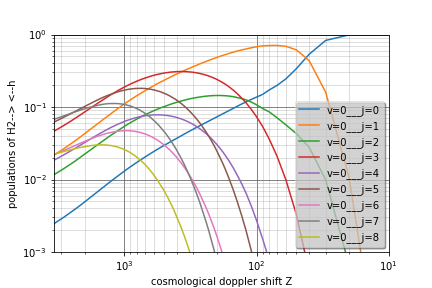
\includegraphics[width=9cm,height=7cm]{levelsh2-h.0.png}
%\caption{Impact du réchauffement sur la température}
%\label{fig:dTCOOL}
\end{subfigure}
\begin{subfigure}{0.5\textwidth}
\centering
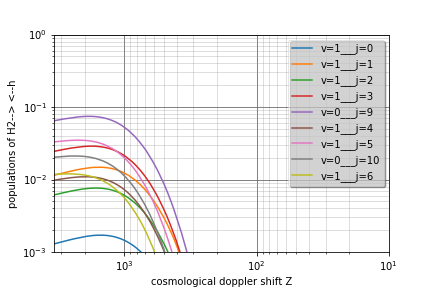
\includegraphics[width=9cm,height=7cm]{levelsh2-h.1.png}
%\caption{Impact du réchauffement sur la température}
%\label{fig:dTCOOL}
\end{subfigure}
\begin{subfigure}{0.5\textwidth}
\centering
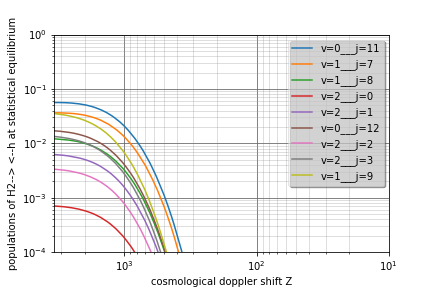
\includegraphics[width=9cm,height=7cm]{levelsh2-h.2.png}
%\caption{Impact du réchauffement sur la température}
%\label{fig:dTCOOL}
\end{subfigure}
\begin{subfigure}{0.5\textwidth}
\centering
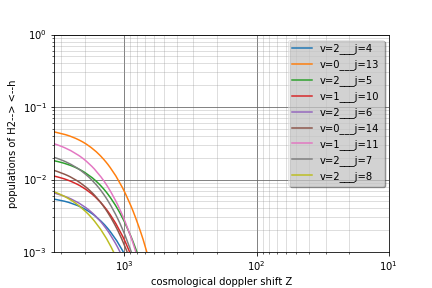
\includegraphics[width=9cm,height=7cm]{levelsh2-h.3.png}
%\caption{Impact du réchauffement sur la température}
%\label{fig:dTCOOL}
\end{subfigure}
\begin{subfigure}{0.5\textwidth}
\centering
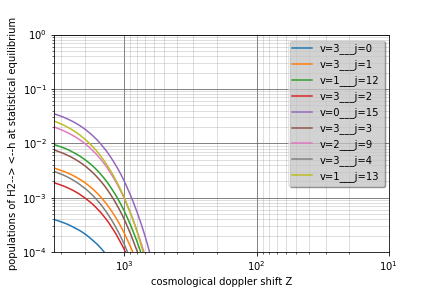
\includegraphics[width=9cm,height=7cm]{levelsh2-h.4.png}
%\caption{Impact du réchauffement sur la température}
%\label{fig:dTCOOL}
\end{subfigure}
\begin{subfigure}{0.5\textwidth}
\centering
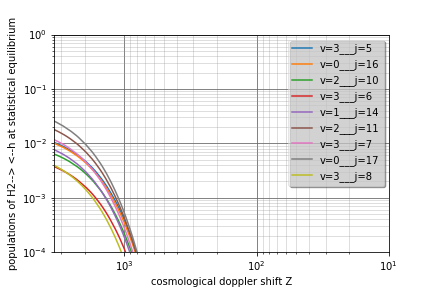
\includegraphics[width=9cm,height=7cm]{levelsh2-h.5.png}
%\caption{Impact du réchauffement sur la température}
%\label{fig:dTCOOL}
\end{subfigure}

\caption{Population des 54 états rovibrationnels de H2 en fonction du décalage vers le rouge cosmologique}
\label{fig:POPH2}
\end{figure}




%\section{Formules utiles de Transfert de Rayonnement}
%\section{Le programme Radex}
\begin{comment}
\makeatletter
\renewcommand\chapter{\if@openright\cleardoublepage\else\clearpage\fi
\thispagestyle{plain}%
\global\@topnum\z@
\@afterindentfalse
\secdef\@chapter\@schapter}
\end{comment}

\begin{thebibliography}{}

\bibitem{Coppola} 
The chemistry of the early Universe, Carla Marla Coppola and Daniele Galli
\\doi:10.1088/2514-3433/aae1b5ch1

\bibitem{Flower} 
The ortho:para $H_2$ ratio in the primordial gas, D. R. Flower and G. Pineau des Forêts
\\Mon. Not. R. Astron. Soc. 316, 901-905 (2000)

\bibitem{PEEBLESBOOK} 
Principles of Physical Cosmology by Phillip James Edwin Peebles 1993
\\Compton-Thompson Scattering page 581, Kompaneets Equation page 603

\bibitem{Galli} 
The Dawn of Chemistry, Daniele Galli and Francesco Palla
\\doi:10.1146/annurev-astro-082812-141029
\\Predicted abundances tableau 2 page 169

\bibitem{Planck2018} 
Planck 2018 results. VI. Cosmological parameters tableau 2 page 15 colonne "TT,TE,EE+lowE+lensing"
\\\url{https://arxiv.org/pdf/1807.06209.pdf}

\bibitem{Weinberg} 
Cosmology, Steven Weinberg

\bibitem{Signes}
Conventions de Signes RG
\\\url{https://en.wikipedia.org/wiki/Einstein_field_equations#Sign_convention}

\bibitem{cours_RG1} 
Relativité Générale, cours de M2, Éric Gourgoulhon
\\\url{https://luth.obspm.fr/~luthier/gourgoulhon/fr/master/relatM2.pdf}
\\Équations de Friedmann page 196, Espace-temps de de Sitter page 200, Espace-temps d’Einstein-de Sitter page 201

\bibitem{cours_RG2} 
INTRODUCTION A LA RELATIVITE GENERALE, Luc Blanchet
\\\url{http://www2.iap.fr/users/blanchet/images/coursRG.pdf}

\bibitem{RADEX} 
RADEX
\\\url{https://arxiv.org/pdf/0704.0155.pdf}
\\Molecular Cooling page 3 équation 16

\bibitem{KWO} 
Physics and Chemistry of the Interstellar Medium, 2007, Sun Kwo
\\Heating and Cooling of Photoionized Regions page 183 équation 6.42

\bibitem{Glover}
Uncertainties in H2 and HD chemistry and cooling and their role in early structure formation, Glover and Abel
\\doi:10.1111/j.1365-2966.2008.13224.x
\\figure 1 page 1634

\bibitem{Gerlich}
Ortho–para transitions in reactive H++H2 collisions, D. Gerlich J Chem Phys 92 2377 (1990)

\bibitem{Lique}
Revisited study of the ro-vibrational excitation of H2 by H: towards a revision of the cooling of astrophysical media, F. Lique MNRAS 453 810 (2015)



\end{thebibliography}


\end{document}